% Template PNSAC newsletter - Article
% Language: Latex
%

% Head

\title{My Days at the Home of the Merlin Engine}
\subtitle{Part 2}
\author{Richard Lodge}

\maketitle

As a new employee, part of my Rolls-Royce induction process was to get
to know some of the production and other R-R facilities around
Derby. After a few weeks of working in the Overheads Department, it
was suggested that it was time for me to go visiting. I was happy to
do this because any opportunity to leave the main accounting office
for a time was to be jumped at.

Rolls-Royce had an internal bus service to take employees between
sites. To catch the bus, an employee went down to the door of the
building and waited for a bus to turn up -- no booking or written
schedule.  I remember my first trip on a company bus. It took me about
half an hour of asking people around how to get to the site I
wanted. I was beginning to realize that much of the operations of R-R
were not written and were passed around by word of mouth and the long
time employees passing on information to the newcomers. Years later,
when working in Northern Canada in native communities I once again
came across this way of handing down unwritten information from the
Elders to the younger people. Before starting my job at R-R I had
believed that the company would be highly organized and disciplined.

I finally managed to find my way to the building I was due to visit.
It was the Foundry. I was introduced to the men who worked in this
evil smelling place. Each of the major engine parts was individually
cast -- there was no automation and a good foundry man could put
together the sand and other parts needed for the casting, mostly from
memory. During WW2 the foundry had concentrated entirely on the
production of military engines, mostly Merlins.  By the time I was
shown round the place there was a bewildering conglomeration of parts
being made for piston, turbo prop and jet engines.

As a young accountant I was expected to understand how the paperwork
and accounting for all this worked. It was a daunting thought and I
left the Foundry feeling overwhelmed.  Throughout my time at R-R I
never became comfortable dealing with the Foundry -- everything seemed
to be so imprecise and up to the skill on the foundry man. Each time I
went there I tried to find out how the men knew how to produce the
same casting every time and the answer was always the same: "Oh, we
just know what to do".  Many of these comments were probably made to
try to make a young guy in a suit from the office look foolish but
they were also largely true!

Sitting in the Overheads Department I saw many of the invoices for
purchases. I could hardly believe it when I saw invoices going through
for payment for dozens of chickens. The delivery was never to the
works canteen but always to the R-R site at Hucknall, a short distance
outside Derby. My supervisor told me that the chickens were fired at
engines on test. I did not believe him until I managed to find a
pretext to visit Hucknall. After another challenge finding the works
bus to get me there, I arrived at the site and was shown round and all
was revealed. Dead chickens ending their time on earth being used to
test the strength of compressor blades in an engine on full power
seemed to me to be a very imprecise way of testing a jet
engine. Another lesson learned -- not everybody was trying to make me
look foolish all the time.

\begin{figure}[htbp]
   \vspace{2em}
   \centering
   %name of the graphic, without the path AND in EPS format:
   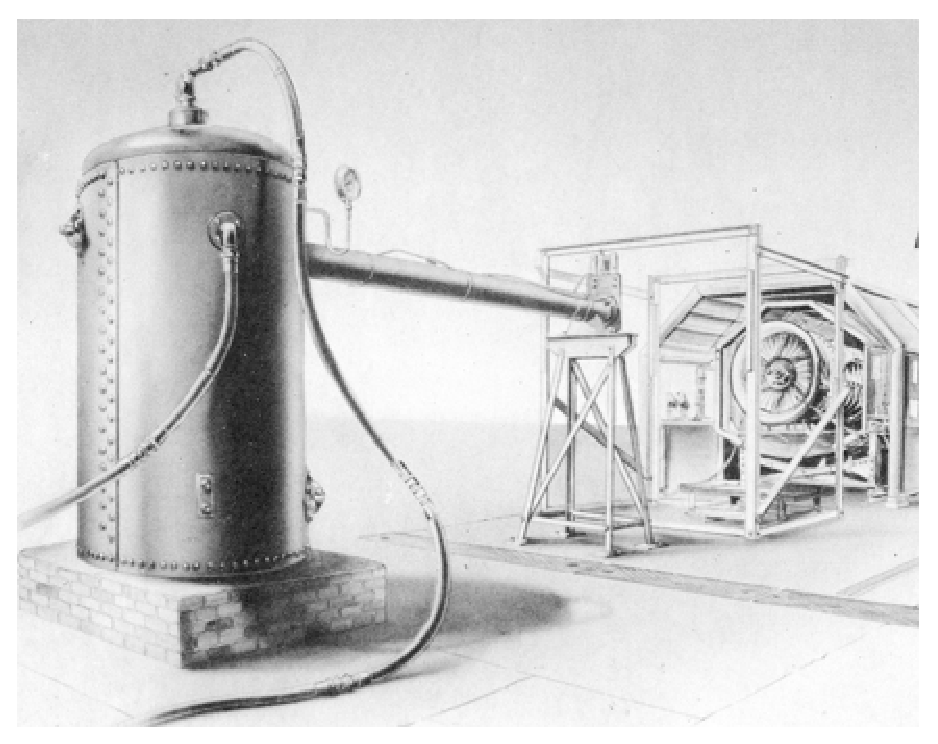
\includegraphics[scale=0.5]{bird_gun.eps}
   %caption of the figure 
   \caption*{\small \em A 1960s chicken gun as used at Hucknall .}
   %label of the figure, which has to correspond to \ref{}:
   \label{fig:birdgun}
\end{figure}

The visits to the various R-R sites around Derby took several months
to complete. I had to have a good reason to leave my office and go
visiting, particularly as I was now working in a departmental
position. Eventually another bus trip to the large new complex at
Sinfin was required or I somehow managed to talk my way into finding
it necessary to go there. Sinfin, among many other things, housed the
main engine test beds and I was curious to find out what happened
there. Unlike the evil smelling Foundry, Sinfin was clean, new and had
plenty of windows.

The men in the test shop told me about the engine testing process. I
was still new to R-R and had a lot to learn. After a while I was asked
if I would like to see an engine on test. Of course I said yes; it
seemed interesting. With little experience I did not realize that an
aero engine on test is nothing much to see. One of the men said he
would take me to a Conway engine on test. He said he would open the
test bed door to let me see the engine and that I would find it
somewhat noisy. He stood behind the door, opened it and let me look
inside at the engine on full power. I now wear hearing aids. Health
and safety were two words not used in those days when many of the men
were used to serving in the war. This was 1960s Britain.

I have always enjoyed travelling and would jump at any opportunity to
travel to a new place. After a few months it was suggested to me that
I should visit the Scottish factory at Hillington near Glasgow. I
asked how I should get there. ``Oh. You might as well fly. There is a
flight every day that leaves in the morning and comes back in the
afternoon.'' I had never flown before.

The UK being a small country, everybody went around by train.  As
usual, I was given very little information and told to get myself to
East Midlands airport early on the appointed morning, where a ticket
would be waiting for me. On this occasion I had the good sense to take
my own car to the airport and did not get lost. I expected to find a
plane waiting, painted in some sort of Rolls-Royce colours. Instead,
after some questioning, I found out that I would be travelling on a
small airline, called British Midland, which ran a service, mainly for
R-R personnel, between the Derby East Midlands Airport, near Derby and
Glasgow factories Airport. Far from being in some interesting plane
connected with R-R, I found that our plane was an old DC3 which had
seen better days.I duly got on the plane and was somewhat nervous
flying on my first flight.

An hour later we arrived in Scotland, also my first trip over the
Border, and I spent the day being shown around the factories and
offices.  I remember very little about the day but vividly remember
the flight back to Derby. It must have been in the winter because it
was getting dark as I boarded the plane around 5.00 pm. Seating was
first come first served and all the old sweats travelling knew what to
do. I ended up on the back row near the cargo area. The main thing I
remember was the crew having a fierce argument about the load on the
plane which was full. The discussion centred around the amount of
cargo which could be taken on the flight. I was quite relieved to get
back to Derby in one piece.

In the next article I will describe how I worked hard to climb the
hierarchy at R-R and learnt in an uncomfortable way some lessons on
people management.


\begin{footnotesize}
    \raggedleft PNSAC\\
\end{footnotesize}

% End of text.

%%% Local Variables: 
%%% mode: latex
%%% TeX-master: main_document.tex
%%% End: 

